% !TEX TS-program = pdflatex
% !TEX encoding = UTF-8 Unicode

% This is a simple template for a LaTeX document using the "article" class.
% See "book", "report", "letter" for other types of document.
\documentclass[11pt,man]{article}
\usepackage[natbibapa]{apacite}
\usepackage{array}
\usepackage{color}
\usepackage{amssymb}
\usepackage{amsmath}
\usepackage{amsfonts}
\usepackage{graphicx}
\usepackage{url}
\usepackage[font={small}]{caption, subfig}
\usepackage[vlined,ruled, noend,linesnumbered]{algorithm2e} 
\usepackage[margin=1in]{geometry}
\usepackage[T1]{fontenc}
\usepackage[utf8]{inputenc}
\usepackage{enumitem}
\usepackage{authblk}
\newcommand\numberthis{\addtocounter{equation}{1}\tag{\theequation}}

\definecolor{Orange}{rgb}{1,0.5,0}
\definecolor{Purple}{rgb}{1,0,1}
\definecolor{Green}{rgb}{0,1,0}
\definecolor{Red}{rgb}{1,0,0}

\newcommand{\todo}[1]{\textsf{\textbf{\textcolor{Red}{todo anyone: [[#1]]}}}}

\newcommand{\todoMatt}[1]{\textsf{\textbf{\textcolor{Orange}{todo Matt: [[#1]]}}}}
\newcommand{\todoKenny}[1]{\textsf{\textbf{\textcolor{Purple}{todo Kenny: [[#1]]}}}}
\newcommand{\todoWei}[1]{\textsf{\textbf{\textcolor{Green}{todo Wei: [[#1]]}}}}
\newcommand{\Expect}{{\rm I\kern-.3em E}}


\def\citeapos#1{\citeauthor{#1}'s (\citeyear{#1})}

\title{Using news media and Twitter to provide a quantitative overview of factors related to the outbreak, successes and failures of the "Arab Spring" }

\author[1]{Kenneth Joseph \thanks{\texttt{kjoseph@cs.cmu.edu}}}
\author[1]{Matthew Benigni \thanks{\texttt{mbenigni@cs.cmu.edu}}}
\author[1]{Wei Wei \thanks{\texttt{weiwei@cs.cmu.edu}}}
\author[1]{Kathleen M. Carley\thanks{\texttt{kathleen.carley@cs.cmu.edu}}}
\author[2]{Mia Bloom\thanks{\texttt{mia\_bloom@uml.edu}}}

\affil[1]{Computation, Organization and Society Program\\ Carnegie Mellon University\\ 5000 Forbes Ave. \\ Pittsburgh, PA, USA}
\affil[2]{Center for Terrorism and Security Studies\\ University of Massachusetts, Lowell\\ Lowell, MA, USA}


\begin{document}
\maketitle
\renewcommand{\baselinestretch}{2}\normalsize

\begin{abstract}

\end{abstract}

\section{Introduction}

Story concepts:

how do discussions change over time and space in the arab spring?

this allows us to compare public focus and news focus

which drives which and how much

in intro: problems with count data, e.g. by showing diffrences in A, other biases

Work to do:

1. Fake data
	create 1 that is positive, does it recover
	random walk data

2. Stop word data
	top 25 nouns, 3 topics (minus man, woman, child, life, gov't)
	top 25 nouns, top 25 adjectives, 3 topics (minus above + young)
3. Re-estimate model with this	

4. Is A term significant? (Raw MLEs) Hyp A term is diff from 1; compare with boring data. Expected: A is negative over time; generally decreasing interest

5. news is fairly stable, Twitter is not. Also some countries with more noise less stable (bigger sigma?)

6. where do news and twitter diverge?  lag plot and just straight time series correlations; maybe think about indices for freedom of press

7. Overall, some high level comparison - event data; corr matrix w/ static data; ``event/outlier  detection'' (or, better, figure out how to get away from this)

8. Case study, Matt

9. lit review

Ideas not for this paper:
	correlate with network changes over time, compare/correlate categories, 


\citeapos{goldstone_cross-class_2011} recent assessment of the drivers of instability and revolutionary success during what has come to be known, for better or worse \cite{gelvin_arab_2015}, as the Arab Spring, suggest that a recurrent causal story played a role in the early revolutionary successes in Egypt, Tunisia and Libya.  Goldstone states that ``virtually all successful revolutions were forged by cross-class coalitions...pitting society as whole against the regime''. He then provides qualitative evidence that the revolutions in three countries were no different.  In Egypt, Tunisia and Libya, previously disparate social groups combined under a united ``cross-class coalition'' of protesters and revolutionaries, which made the revolutions significantly more likely to succeed.

In later work, \citeauthor{goldstone_bringing_2013} \citeyearpar{goldstone_bringing_2013} suggests that several additional predictors were important in determining whether or not a particular government was ultimately overthrown.  Chief amongst these predictors, he argued, was the structure of the overarching regime had a strong impact on whether or not the government was ultimately overthrown.  Goldstone defines a \emph{personalist} regime as one in which a single individual – who may have begun as an elected leader, or head of a military or even party regime – takes total or nearly total control of the national government. He then provides qualitative evidence for his believe that ``the single best key to where regimes in MENA have been overturned or faced massive rebellions is where personalist regimes have arisen''.
 
Goldstone's critiques are two of many articles to consider what may have led to the revolutions that spread throughout the MENA region and whose effects still continue to reverberate globally today. One factor of primary interest was the use of social media, which was originally suggested by popular media to be the sole cause of the spread of the revolution. At this point, it is almost common knowledge that this emphasis on social media as a \emph{cause} of the revolutions is overblown \citep{bruns_arab_2013,goldstone_bringing_2013,comunello_will_2012}. However, many scholars have pointed to the fact that the use of social media may have aided certain aspects of the revolutions in important ways for different people  \citep{galle_who_2013,starbird_how_2012,lotan_revolutions_2011,tufekci_social_2012}.  This fits with the current understanding of the causal structures involved,  as scholars now suggest that a breadth of heavily intertwined issues came together in a unique and unpredictable fashion to provide the conditions necessary for the spread of both successful and unsuccessful revolt and protest throughout the region. 

In contrast to work considering the causal role that social media played in the revolution, recent work has suggested that data from social media data may help to inform this broader understanding of how the revolutions grew and spread \citep{}.  This use of social media data takes as a given that these tools were used in some way during the revolution and goes beyond this in assuming, via the well-worn notion of media multiplexity \citep{}, that causal processes of the revolution which existed ``offline'' are likely to have played out ``online'' as well.  Such work has shown that, for example, X, Y, Z. Similarly, recent work has suggested that data from news media during the time of the Arab Spring also may be of use in better understanding these processes \citep{joseph_arab_2014,pfeffer_rapid_2012}. Combined, efforts with social and news media data from the Arab Spring have shown the value in using this data to a) provide evidence for or against prior hypotheses presented in the literature using quantitative metrics on large sets of data, and b) use the available data to generate new or more nuanced understandings of the incredibly complex web of factors that have been implicated in a causal role.

The present work provides an example of how social and news media data can be used in each of these two ways. First, we extract quantitative evidence for the assertions of \citeapos{goldstone_cross-class_2011}. More specifically, we consider the following two claims made by Goldstone and consider the extent to which they played out in social and news media across Egypt, Libya and Tunisia as well as fourteen other nations in the MENA region:
\begin{itemize}
	\item {\bf H1}: \emph{If a country has more disparate groups, it is more unstable}
	\item {\bf H2}: \emph{If these groups align under a revolutionary cause, the revolution is more likely to succeed}
\end{itemize}

These two hypotheses are directly quantifiable via a combination of social media and news data and external indicators based on expert opinion.  \todoKenny{In order to evaluate {\bf H1}, we consider ... In order to evaluate {\bf H2}, we ...}

In the second part of the paper, we provide a characterization of how social media use may have differed in nations with personalist regimes as opposed to nations with other types of regimes discussed by Goldstone. We combine a host of metrics measured on both news and social media and use a variety of statistical techniques to extract differences.  \todoKenny{We find XYZ. This leads to an interesting extension/correlary/etc of Goldstone in that XYZ...}

%From Ghita: if you talk about arab you don’t mean iran

%These concerns include the fact that ``data-driven'' analysis often suffers from post-hoc conclusions which substantially increase the number of ``researcher degrees of freedom'', even if unintentionally, in the analysis \cite{}. 

	%\item {\bf H3}: (term network) if media representation shows protestors as representative of the whole society, rather than as one particular group seeking partisan advantages for itself, revolution will be more successful
 	%\item Attempt to quantify how Mohammad Bouazizi’s setting himself on fire spreads across normally disconnected factions within the Twitter data in Tunisia from Dec 2010 – Feb 2011.
 	%\item I think we could use our religiosity terms to measure factionalism/sectarianism at the onset of Egypt’s protests.  Both counts and term networks could be useful.

%
%\subsection{My list of covariates}
%
%\begin{enumerate}
%    \item {\bf Regime-based}
%        \begin{enumerate}
%            \item religious freedom indices
%            \item personalist/not \cite{goldstone_bringing_2013}
%            \item wealth (particularly oil) \cite{goldstone_bringing_2013}
%            \item Twitter/News mentions of regime (of some kind) - sentiment?
%            \item Twitter/News revolution/insurgent/violence or adaptation terms
%        \end{enumerate}
%    \item {\bf International relations} 
%        \begin{enumerate}
%            \item international network position
%            \item international Twitter/News network position
%        \end{enumerate}
%    \item {\bf Population indicators } 
%        \begin{enumerate}
%            \item Twitter/news geospatial spread
%            \item Religious indices
%            \item Ethnic diversity / group indicators
%            \item Twitter/news mentions of ethnic group
%            \item Twitter/news attention / network position
%            \item Twitter/news ``class'' cohesiveness \cite{goldstone_cross-class_2011}
%            \item Twitter/news ``class'' spread \cite{goldstone_cross-class_2011}
%        \end{enumerate}
%\end{enumerate}
%
%


\section{Related work}

Also this special issue: \url{http://onlinelibrary.wiley.com/doi/10.1111/jcom.2012.62.issue-2/issuetoc}

\citep{mishra_enthusiasm_2014}



\section{Our To-dos}

\begin{enumerate}
\item Change/iterate this document to something we actually think we can do
\item Figure out what is up with that jump in the Twitter data
\item Motivation for the article
\item Related Work
\item Method for correlation analysis for each of the three levels
\item Run Netmapper, etc
\end{enumerate}


\section{Case Study}

Our case study is divided into two sections. In the first, we focus on understanding how countries cluster in thematic space, particularly with respect to protest. In the second, we consider in greater detail how patterns in the protest theme differentiated by media provide support for claims explored by \cite{cottle_media_2011}.

\subsection{Connecting countries and themes}

\begin{figure*}[th]
	\centering
	\begin{tabular}{cc}
		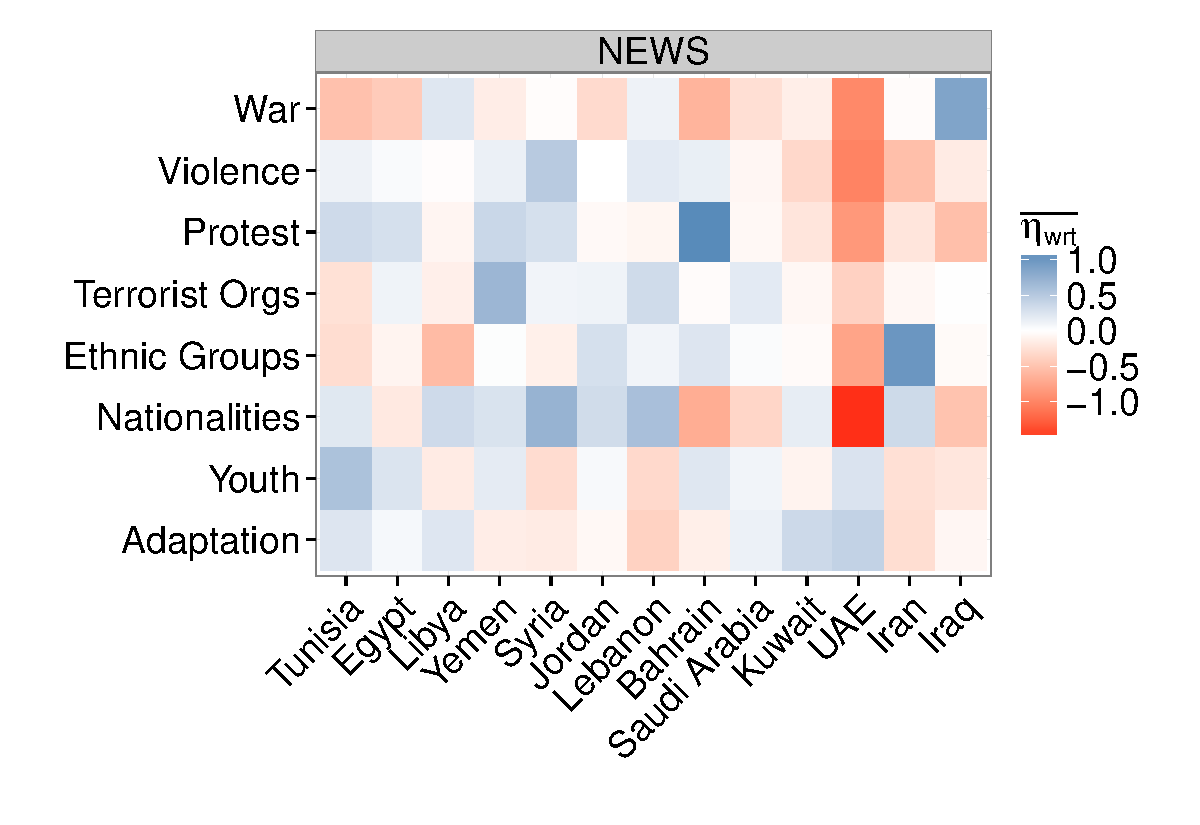
\includegraphics[width=.5\textwidth]{imgs/activity_topics_news} &
		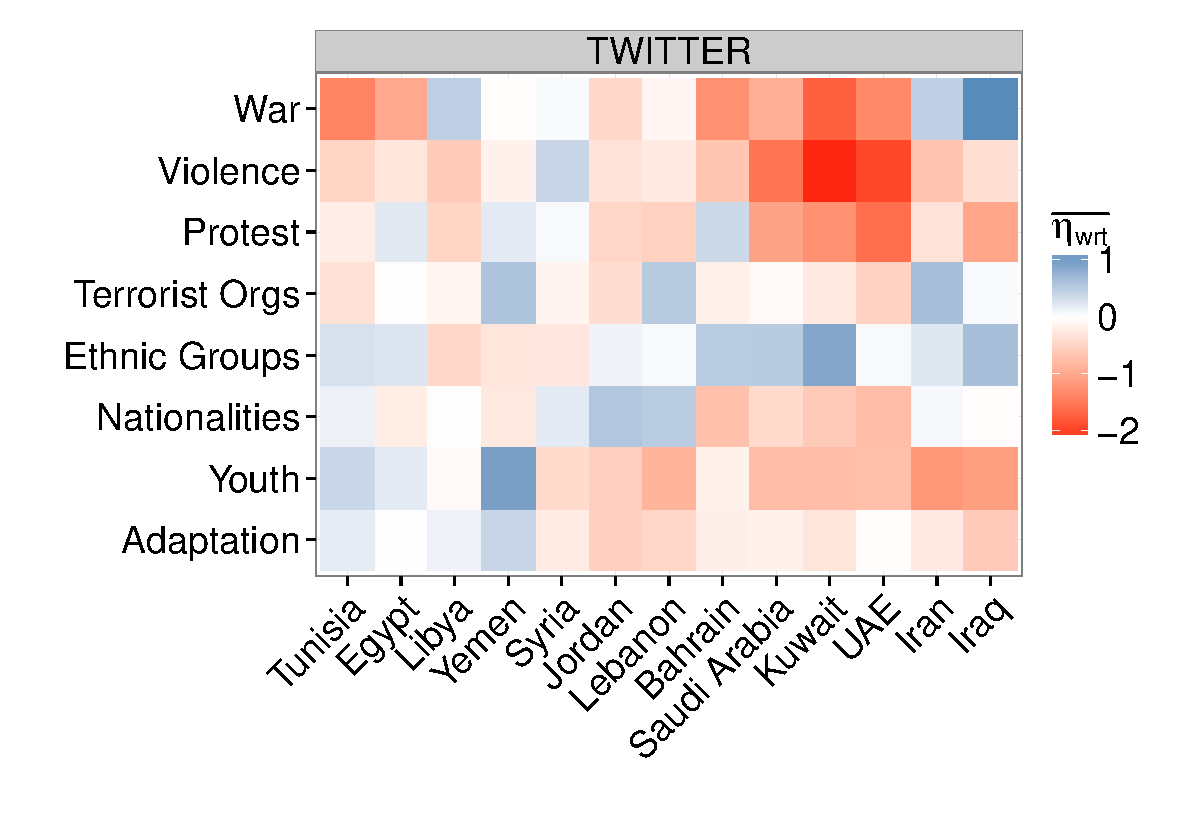
\includegraphics[width=.5\textwidth]{imgs/activity_topics_twitter} \\
	\end{tabular}
	\caption{Mean activation rate over all months for each country and category combination.  The higher the value above 0, the darker the blue. The lower the value below 0, the darker the red. }
	\label{fig:overall}
\end{figure*}


Figure \ref{fig:overall} shows two plots, one for news (left) and one for Twitter (right). Each plot depicts a heatmap of the mean activation values ($\overline{\eta_{w,r,t}}$) over all months for each country/theme combination. The higher the mean activation score above zero for a particular theme/country combination, the darker blue the square. The lower the value below zero, the darker the red. Additionally, note that values are interpretable relative to global activity of each topic/country combination. That is, the dark blue square in the top right of the Twitter plot shows that, on average, relative to other countries, discussions of war were more frequent in Iraq than the discussion of other topics. 

Figure \ref{fig:overall} suggests two fascinating patterns in how countries clustered along themes explored here. First, we considered how countries clustered along perhaps the most interesting theme with respect to the Arab Spring, that of protest.  Figure~\ref{fig:overall} shows that for countries in which protests occurred at relatively low levels (Iran, Iraq, Saudi Arabia and the UAE), discussion of protests were low in both the news and Twitter data. Interestingly,  however, even in countries where relatively high levels of protest occurred, a distinction can be made in the level of discussion of protest between countries where revolutions are still ongoing or succeeded in overthrowing the government (Egypt, Yemen, Tunisia, Libya, Bahrain and Syria) versus those where little social change occurred (Jordan, Kuwait, Lebanon).  In all but Libya, countries where social change followed protests showed positive (above zero, on average) levels of discussion about protest in the news media data. In contrast, countries where protests failed to produce significant results showed negative activation rates for this theme, on average, across time.  In the Twitter data the same patterns hold, although discussion of protest in Tunisia, who's government fell before the beginning of our data collection, is also negative.

\begin{figure}[t]
	\centering
	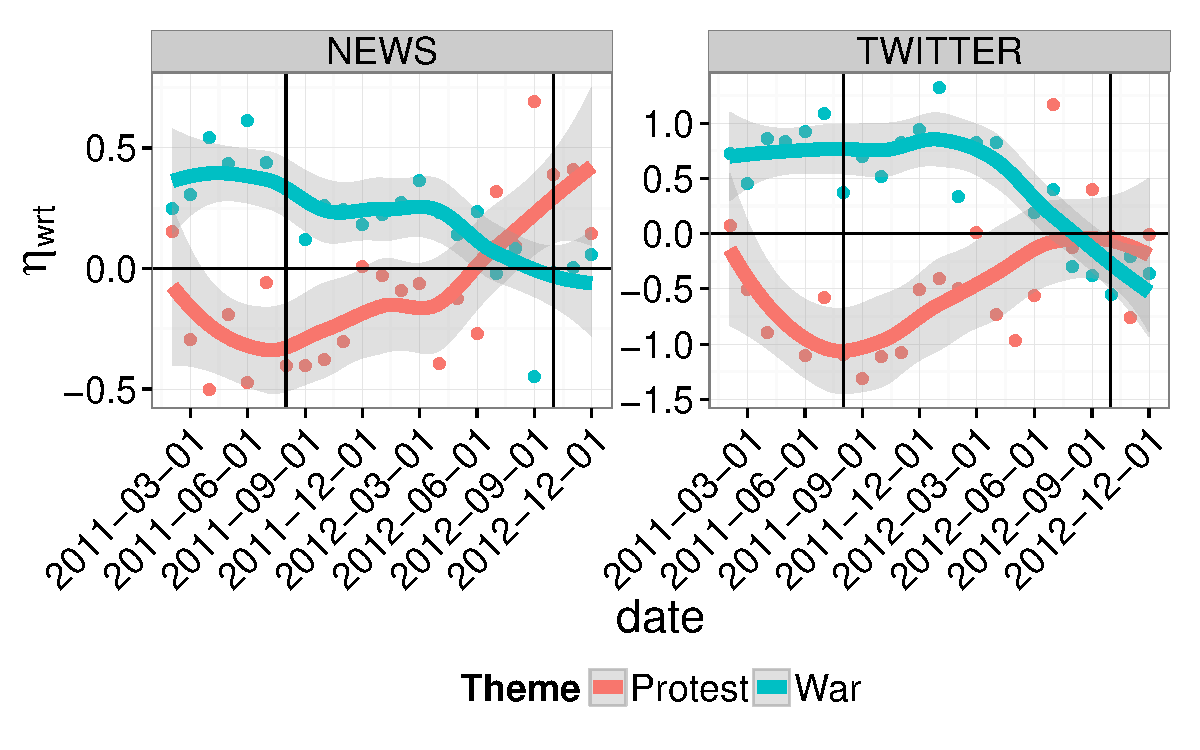
\includegraphics[width=.5\textwidth]{imgs/lib_protest_viol}
	\caption{Relationship between the protest and war themes over time in Libya. Points represent estimates from the model, nonparametric smoothed estimates with 95\% confidence intervals are provided as lines to ease visual observation of trends.}
	\label{fig:prot_viol}
\end{figure}

In sum, results show that in both Twitter and news media, levels of discussions about protest clustered into countries in which important social change occurred during the period, where positive activation scores for protest were observed, and countries where little or no social change occurred, where negative activation scores were seen. The lone exception to this categorization was Libya, where a six month civil war eventually led to the downfall of the ruling regime. We can understand why low levels of discussion on the subject of protest occurred by looking at the way in which protest was discussed over time in Libya. Figure~\ref{fig:prot_viol} shows the activation rates of the categories protest and war over time in Libya. The first vertical black line represents, approximately, the point at which the ruling regime was overthrown, the second black line represents the attack on the U.S. consulate in Benghazi.  As we can see, the focus in Libya on protest may largely have been mediated by a focus on the civil war and its aftermath.  However, as unrest grew again in the face of complaints about the new regime, we do see a renewed trend towards protest, which could be seen as an initial indicator of a return to civil unrest.  This intricate relationship between discussions of war and protest is of particular interest in understanding how unrest leads to organized violence.
 
\begin{figure}[t]
	\centering
	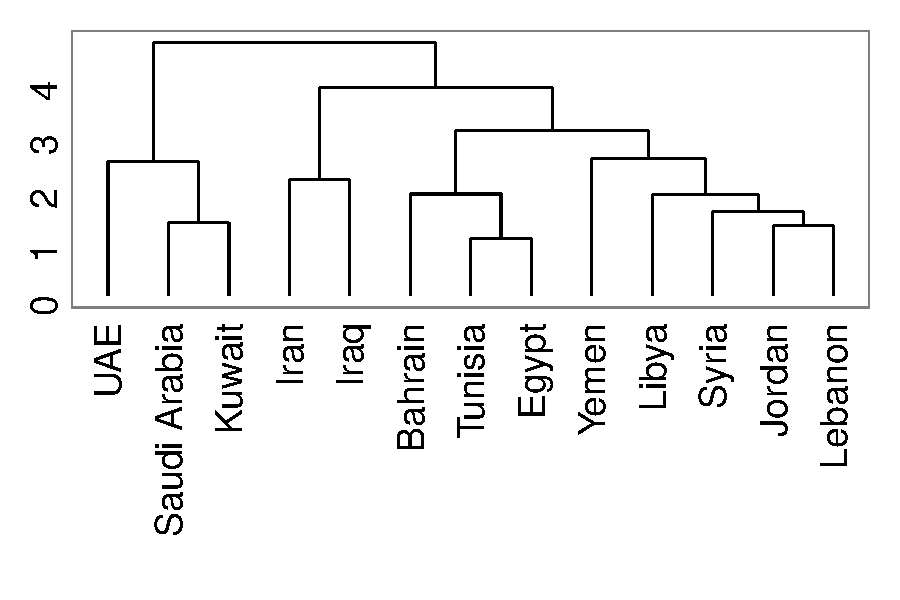
\includegraphics[width=.5\textwidth]{imgs/country_dendro}
	\caption{Hierarchical clustering of our 13 countries based on mean activation levels across all categories for both news and Twitter }
	\label{fig:clust}
\end{figure}

Figure~\ref{fig:overall} also suggests there exists clusters of countries that exist at a larger level than simply distinctions across protests.  To better evaluate the extent to which this clustering exists, we perform a standard, complete-linkage, agglomorative clustering, where each country is represented by sixteen features (the eight categories shown in Figure~\ref{fig:overall} for both news and Twitter). Figure~\ref{fig:clust} presents a dendrogram of the resulting clustering.  Figure~\ref{fig:clust} shows that the oil-rich nations of Saudi Arabia, Kuwait and UAE, where little social change occurred, showed similar thematic structures.   Similarly, nations with which the United States has the strongest tensions, Iran and Iraq, cluster together.  Figure~\ref{fig:clust} shows that these five countries  are heavily separated in thematic content from nations where social change occurred, although they are also separated from perhaps the more similar nations of Lebanon and Jordan.  Within the cluster holding nations where large-scale social change occurred, we observe that Tunisia and Egypt are the most tightly connected, an indication of the extent to which these two revolutions were tied together. 

\subsection{Temporal patterns in protests}

\begin{figure}[t]
	\centering
	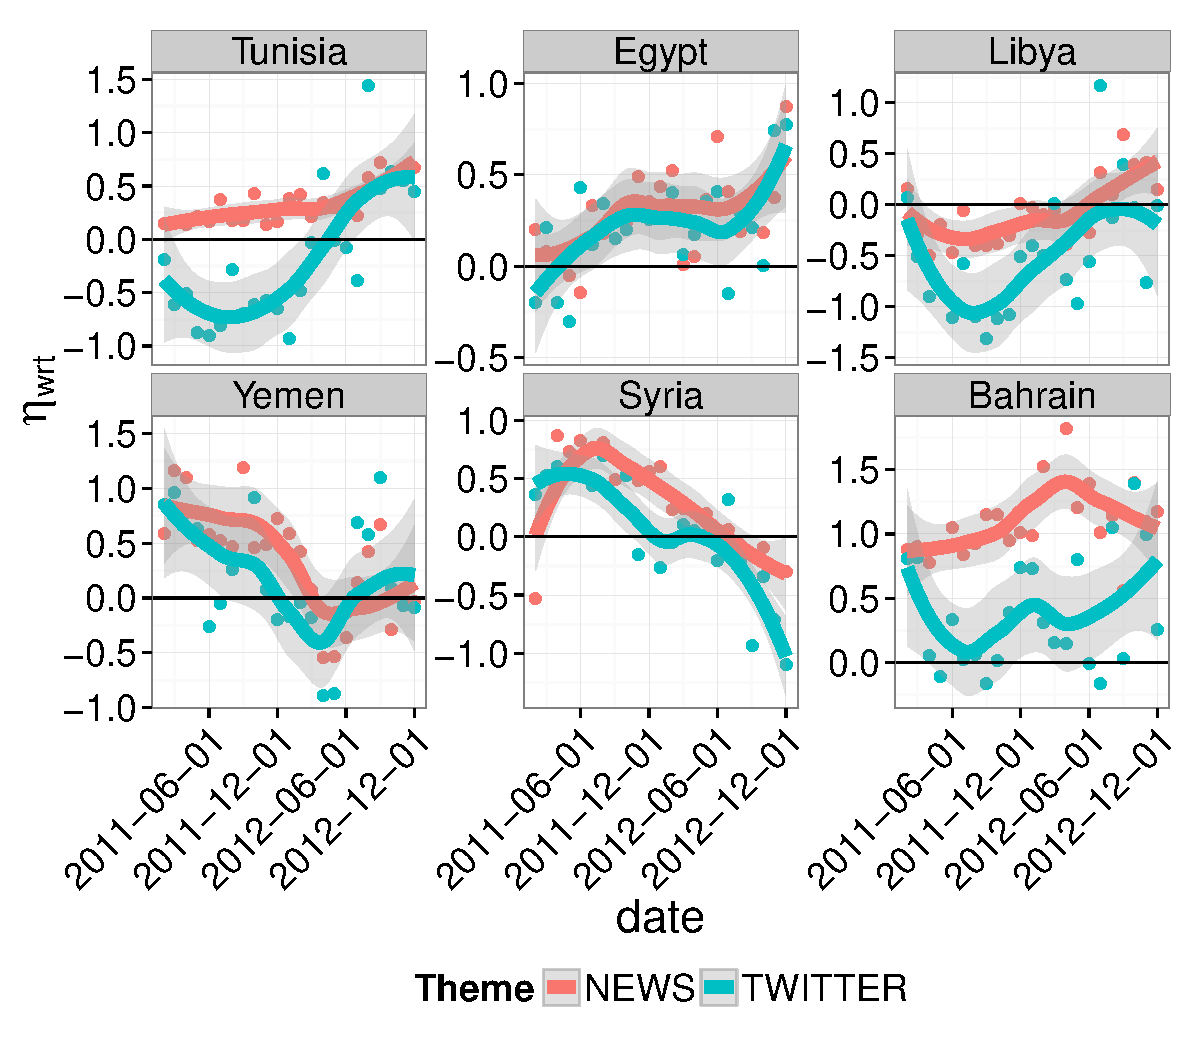
\includegraphics[width=.5\textwidth]{imgs/cottle}
	\caption{Activation Rates of protest over time for six countries of interest.  Points represent estimates from the model, nonparametric smoothed estimates with 95\% confidence intervals are provided as lines to ease visual observation of trends.}
	\label{fig:cottle4}
\end{figure}

Having noted that important clustering appears in average levels of activation with respect to protests, we turn now to how temporal patterns of protest played out in both news and Twitter for nations where high levels of social change occurred. Figure~\ref{fig:cottle4} illustrates activation rates for the theme of protest in news media and Twitter for Bahrain, Egypt, Libya, Syria, Tunisia and Yemen. Our findings, even over time, are consistent with the idea presented by \cite{cottle_media_2011} that new media played an important role in discussions of protests during the Arab Spring.  Perhaps more interestingly, \cite{cottle_media_2011} also argues that the relationship between social media and news media facilitated international recognition and protest legitimization, and provided human rights surveillance.  Our analysis is consistent with this assertion.  In contrasting results for Egypt, with its partially free press, to more restricted countries like Syria, Tunisia, and Bahrain, we observe that states with more oppressive regimes tend to show less of a relationship between social and news media. However, even in the more oppressive regimes, uptakes in Twitter activation with respect to protest always lead to corresponding changes in news activation rates which implies a strong interaction between the two media types. This relationship between news media and social media activation rates reinforce \citeapos{cottle_media_2011} premises. 

Since these clusters of countries we extract in this section are based on both news and Twitter, they cannot be attributed to just a western view of similarity among the countries.  Rather, they reflect some underlying commonality in the way information about and from the these countries is presented across a diverse media landscape.  On the one hand, these clusters show which countries have a common media profile and so, to an extent, a common pattern of media usage by the population.  On the other hand, these clusters may indicate how countries might be similarly influenced by a media campaign.  

%we pr little quantitative research exists analyzing the interaction between news and social media throughout the Arab Spring.   \citet{cottle_media_2011} presents the most comprehensive study to date and presents well argued hypotheses pertaining to the complex interactions between the two types of media and their implications for social change in MENA.  However, he does so with little empirical evidence and calls for ``careful documentation and comparative analysis in the months and years ahead.''  The following section will highlight how activation rates support or refute several of his assertions. 

%\todo{develop fig:cottle4. Decription: topic: protest countries: Bahrain, Egypt, Libya, Syria, Tunisia, Yemen. That depicts smoothed activation rates over time.  Similar to the blah2 plots}

% \todo{ I was not able to show a relationship between news v twitter correlation with either freedom of the press index or internet saturation.  I think there are a couple observations making this problematic.  First, very small set.  Protest and violence are only relatively important topics in a few countries, and not all of them are of equal interest in english speaking news media. I'm open to suggestions}


%	
%	\begin{figure*}
%		\centering
%		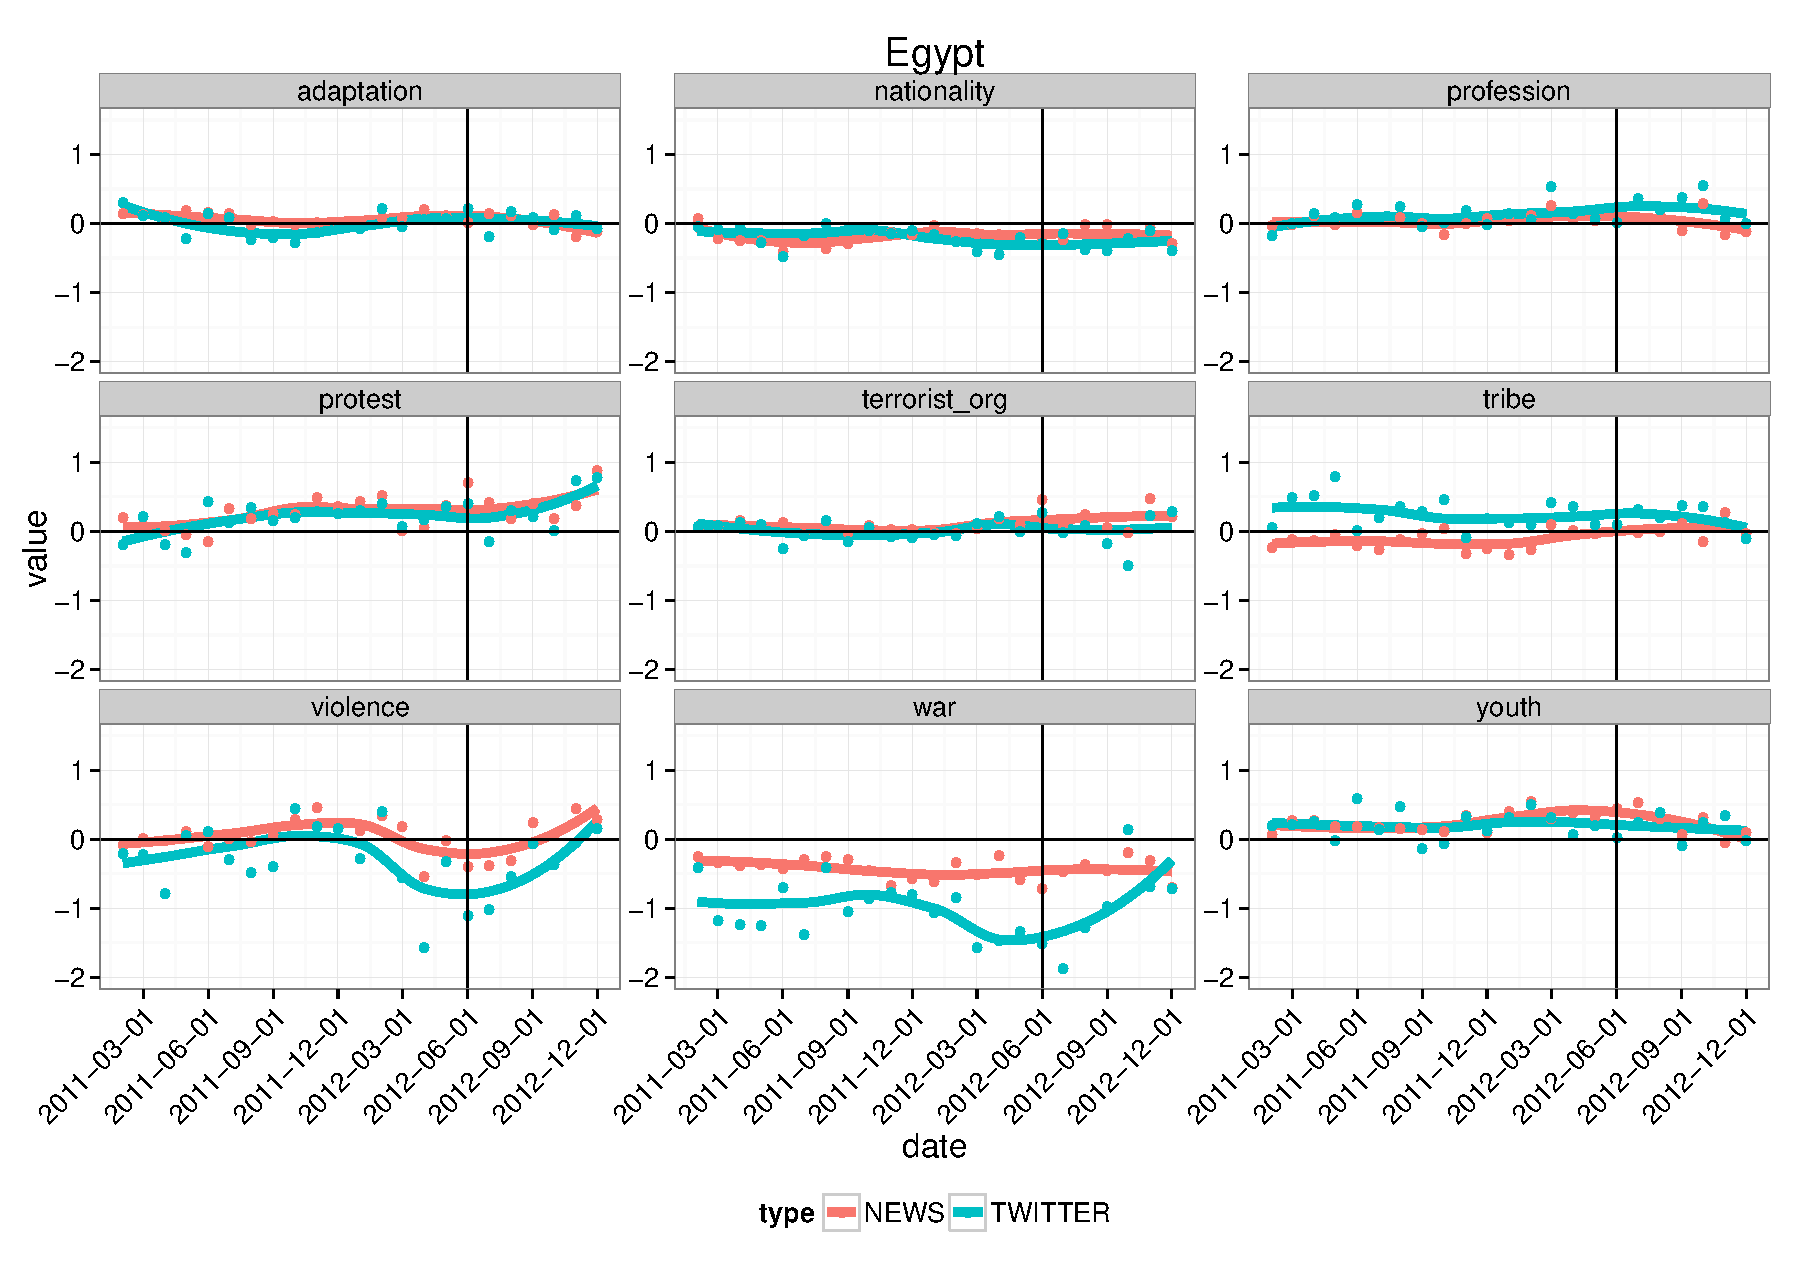
\includegraphics[width=\textwidth]{imgs/egypt.pdf}
%		\caption{Egypt: Black line is when Morsi is elected}
%		\label{fig:egypt}
%	\end{figure*}
%	
%	\begin{figure*}
%		\centering
%		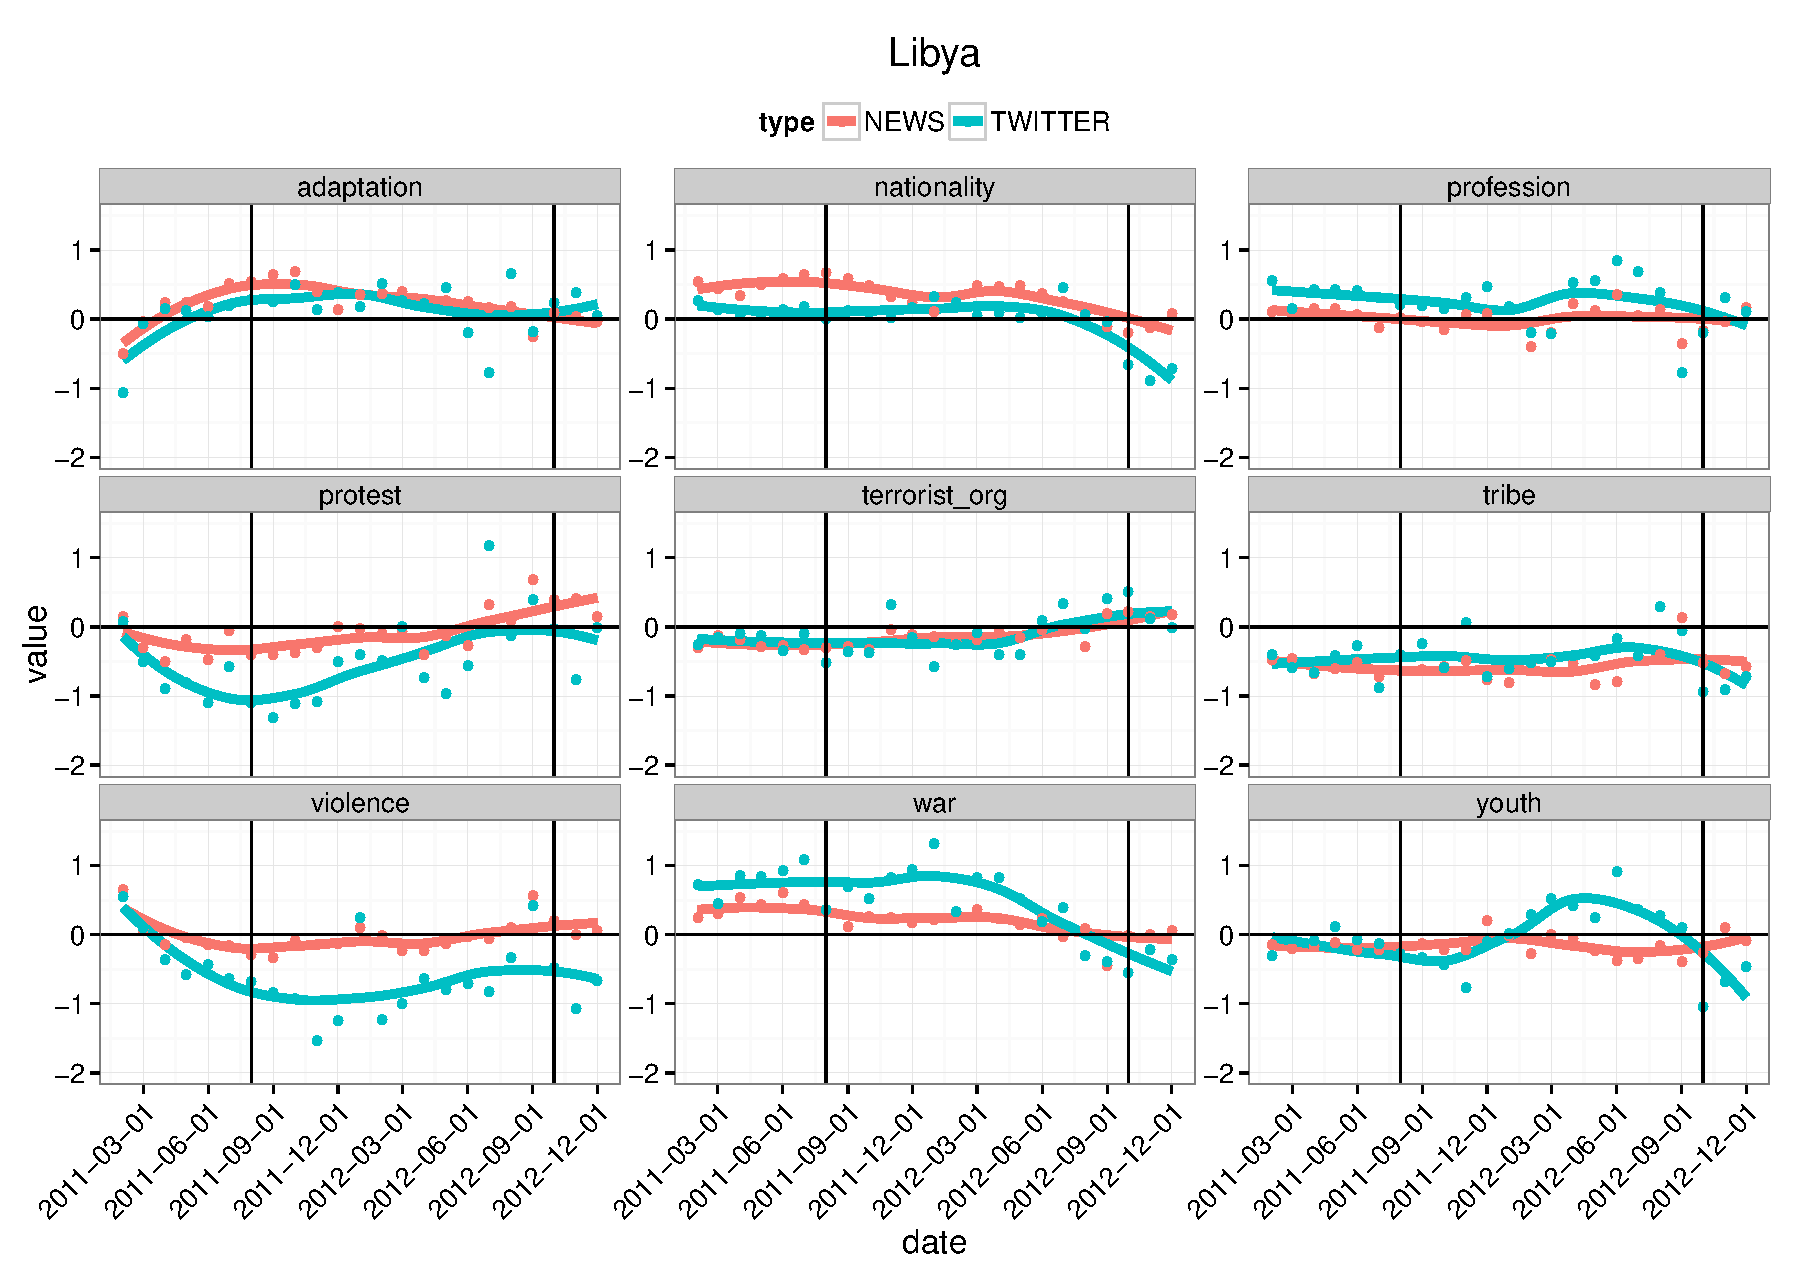
\includegraphics[width=\textwidth]{imgs/libya.pdf}
%		\caption{Libya: Black lines are death of Gaddafi and Benghazi }
%		\label{fig:libya}
%	\end{figure*}
%	
%	\begin{figure*}
%		\centering
%		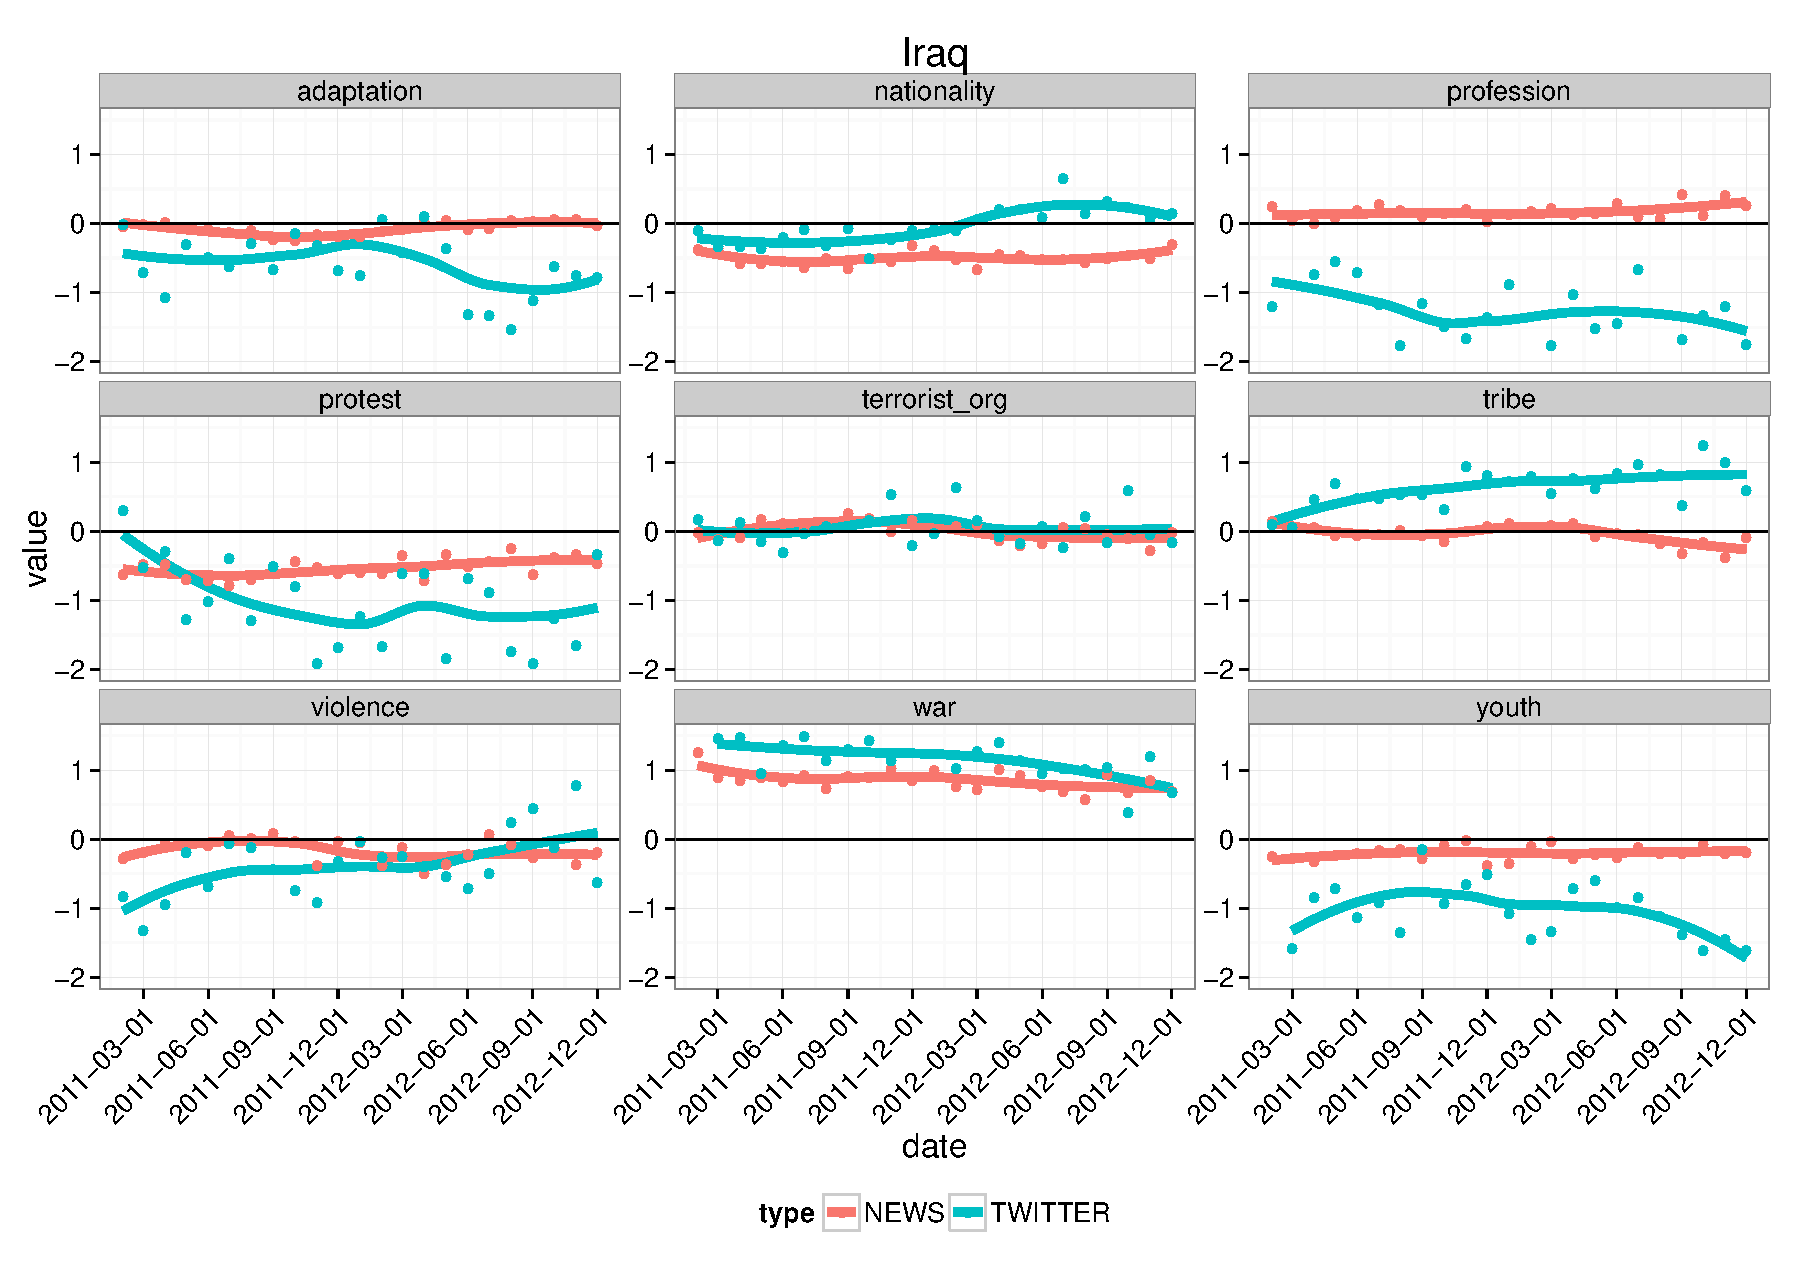
\includegraphics[width=\textwidth]{imgs/iraq.pdf}
%		\caption{Iraq}
%		\label{fig:iraq}
%	\end{figure*}
%	
%	
%	\begin{figure*}
%		\centering
%		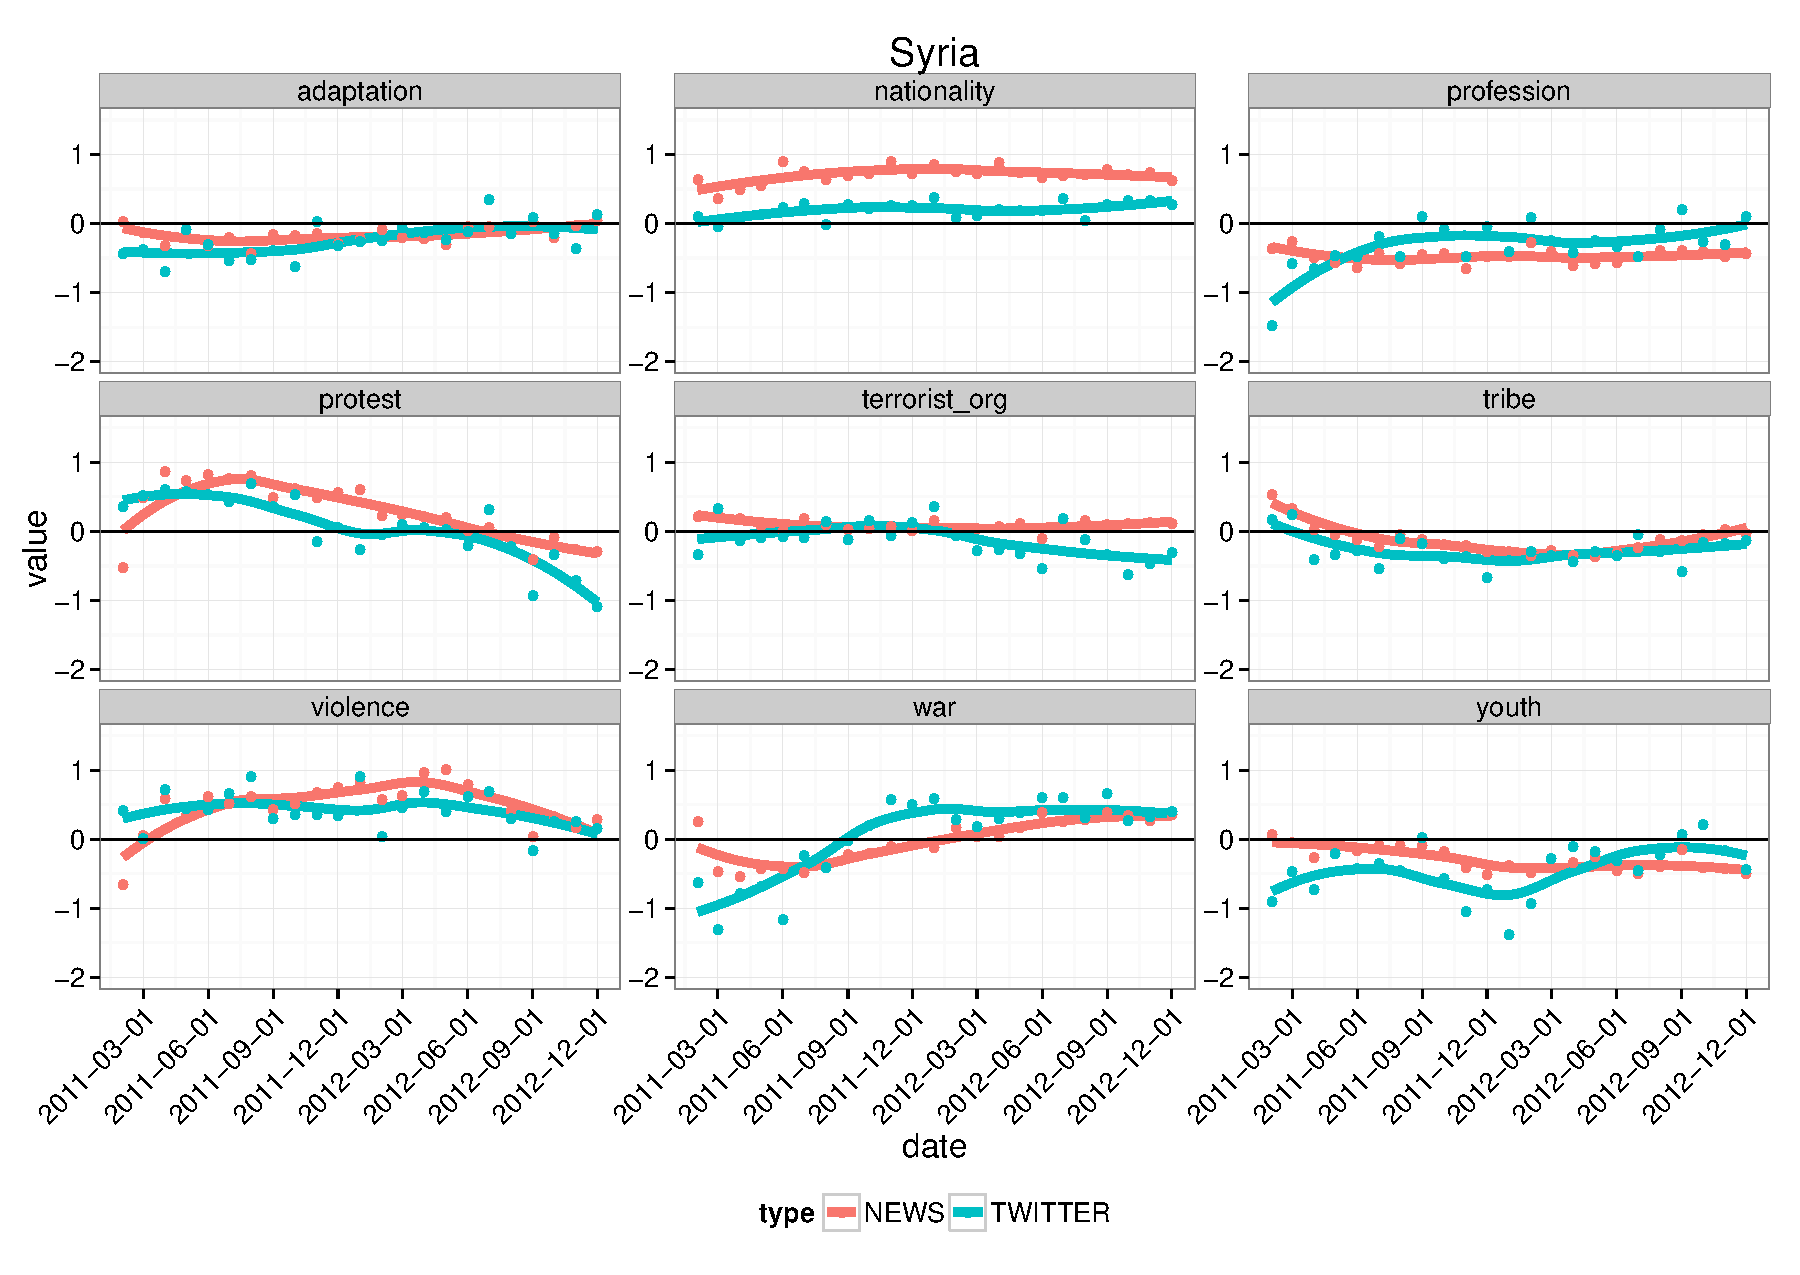
\includegraphics[width=\textwidth]{imgs/syria.pdf}
%		\caption{Syria}
%		\label{fig:syria}
%	\end{figure*}
%	 







\section{Conclusion}

Our analysis is cowith the acknowledgement of the rash of recent claims over the methodological trapdoors that exist within this type of data \cite{tufekci_big_2014,ruths_social_2014,joseph_approach_2014,morstatter_is_2013}. While these issues are not to be ignored, the present work utilizes cautious, nuanced analysis techniques which account for, or at least admit, these possible biases. 


\bibliographystyle{apacite}
\bibliography{mybib} %your bib file


\end{document}
